\chapter{Model}
\label{chap:model}

We can understand the specifics of demodularization by describing it as an algorithm for a simple language with a well defined semantics.
The simple language models the existing Racket module system.
We describe a small-step operational semantics (a series of syntactic rules) that define how the language works.
We also define a compiled version of the language that mirrors the compiled version of Racket.
Next, we describe how the demodularization algorithm works as a metafunction over the language.
Finally, we show that programs before and after demodularization produce the same results.

\section{A Module Language}
The \emph{mod} language (Figure~\ref{fig:source-lang}) contains only the features necessary to write modular programs where it is possible to observe the effects of module evaluation order.

\begin{figure}
\centering
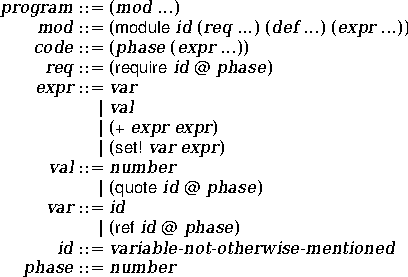
\includegraphics{figures/source}
\caption{\emph{mod} language grammar}
\label{fig:source-lang}
\end{figure}

A program in \emph{mod} consists of a list of modules that can refer to each other.
Each module has a name, any number of imports, any number of definitions, and a body of code. 
All definitions in a module are exposed as exports to other modules, but to use definitions from another module, the program must import it through a \texttt{require} expression.
Both \texttt{require} and \texttt{define} expressions have phase annotations; this simulates the interactions between modules in a language with macros without requiring a model of macro expansion.
The language includes variable references, numbers, addition, and mutation.
Mutation makes module evaluation order observable, and addition represents the work that a module does.
In addition to numbers and variables, there are two special forms of values and references that model the interaction of macros with the module system.
A \texttt{quote} expression is like a reference to syntax at runtime.
A \texttt{ref} expression is like a macro that can only do one thing: refer to a variable at a phase.

\section{Compilation}

We have to compile \emph{mod} programs before demodularizing them, just like in the Racket implementation.
In Racket, compiling expands all macros in a program and changes definitions and variable references to refer to memory locations.
In \emph{mod}, compiling eliminates \texttt{ref} expressions, turns definitions into \texttt{set!} expressions, changes variable references to include module information, and sorts code into phases.
Compilation in both cases still leaves behind a relatively high-level language, but the language is free of syntactic extensions.
This is important for demodularization because otherwise macro expansion would have to be part of the algorithm, which would complicate it and possibly duplicate work.
The grammar in Figure~\ref{fig:compiled-lang} specifies the compiled language for \emph{mod}.

\begin{figure}
\centering
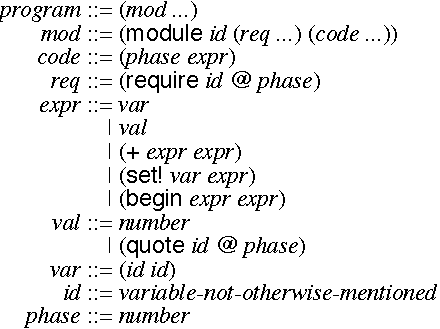
\includegraphics{figures/compiled-lang}
\caption{Compiled language grammar}
\label{fig:compiled-lang}
\end{figure}

The grammar no longer has definitions, all variables now include module references, and code is sorted into phases.
The actual compilation function is not relevant to demodularization.

\section{Evaluation}

We evaluate the compiled language using a small-step reduction semantics. 
Because the reduction rules are syntactic, we extend the compiled language further with evaluation contexts, a heap representation, and a stack representation to keep track of the order to instantiate modules.
These extensions are in Figure~\ref{fig:compiled-eval-lang}.
An expression of the form:
\[
  (\sigma\ /\ (program\ /\ ((id\ phase)\ \ldots)\ /\ ((id\ phase)\ \ldots)))
\]
represents the state of the machine during evaluation.
$\sigma$ represents the heap of the program, and when evaluation finishes represents the output of the program.
The list of modules is the code of program in the compiled language.
The first list of \emph{(id phase)} pairs is the list of modules to evaluate, and the second list is the modules that have already been evaluated.

\begin{figure}[h]
\centering
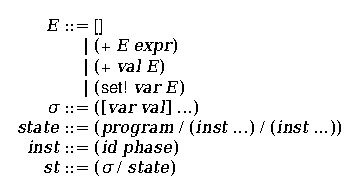
\includegraphics{figures/compiled-eval-lang}
\caption{Extensions to compiled language grammar}
\label{fig:compiled-eval-lang}
\end{figure}

The reduction rules in Equations~\ref{eq:module-require}--\ref{eq:module-done-already} evaluate a compiled program that starts with an empty heap, the program code, a stack that contains the identifier of the main module at phase 0, and an empty completed module list. 
Evaluation proceeds by adding required modules to the evaluation stack and executing code of modules in the order they appear on the evaluation stack when there are no more requires left.

\begin{equation}
  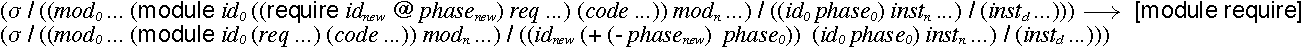
\includegraphics[width=0.9\textwidth]{figures/eval-reduction0}
  \label{eq:module-require}
\end{equation}

% TODO: explain that phases are relative
The rule in Equation~\ref{eq:module-require} matches a program with a \texttt{require} expression in the module at the top of the evaluation stack and evaluates it by removing the \texttt{require} expression from the module and pushing the required module onto the evaluation stack with the phase shifted by the difference between the current module's relative phase and the required phase.
The $\ominus$ is not part of the language and represents the prefix version of the math function minus.
The current module is still on the stack and will continue evaluating after the required module is done evaluating.
The subsequent rules all apply only when the phase relative to the main module is zero.

\begin{equation}
  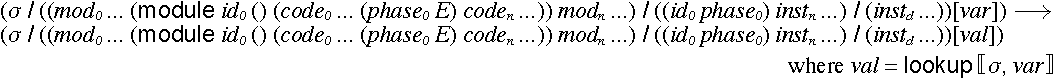
\includegraphics[width=0.9\textwidth]{figures/eval-reduction1}
  \label{eq:var-ref}
\end{equation}

The rule in Equation~\ref{eq:var-ref} looks up a variable in the heap and replaces the variable with its current value.
The lookup function is a simple list lookup function that matches the variable name with its occurence in the heap. 

\begin{equation}
  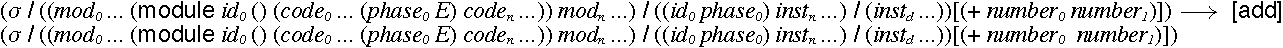
\includegraphics[width=0.9\textwidth]{figures/eval-reduction2}
  \label{eq:add}
\end{equation}

The rule in Equation~\ref{eq:add} replaces an addition expression of numbers with the result of computing their sum.
The $\oplus$ represents the prefix version of the math function plus.

\begin{equation}
  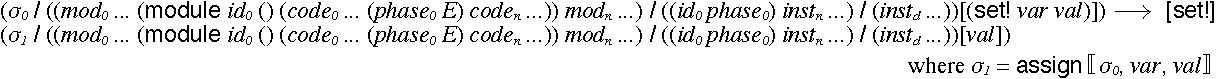
\includegraphics[width=0.9\textwidth]{figures/eval-reduction3}
  \label{eq:set}
\end{equation}

The rule in Equation~\ref{eq:set} installs a value for a variable into the heap and reduces to the value.
The assign function either replaces the existing value for a variable in the heap or installs a new entry in the heap if it does not exist already.

\begin{equation}
  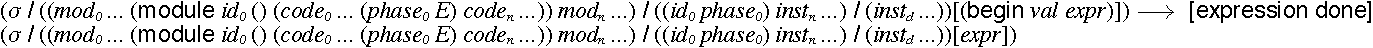
\includegraphics[width=0.9\textwidth]{figures/eval-reduction4}
  \label{eq:expression-done}
\end{equation}

When an expression is a \texttt{begin} with a value in the first position, the rule in Equation~\ref{eq:expression-done} removes the value and replaces the \texttt{begin} expression with the expression in the second position.

\begin{equation}
  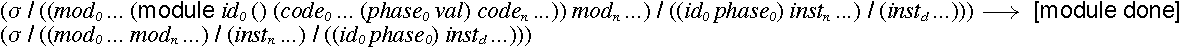
\includegraphics[width=0.9\textwidth]{figures/eval-reduction5}
  \label{eq:module-done}
\end{equation}

When there are no more expressions left in a module, the rule in Equation~\ref{eq:module-done} applies by removing the module from the program and placing a reference to it in the list of finished modules.

\begin{equation}
  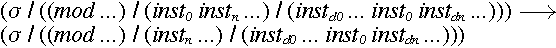
\includegraphics{figures/eval-reduction6}
  \label{eq:module-done-already}
\end{equation}

The rule in Equation~\ref{eq:module-done-already} applies when the current module on the stack is in the finished list, so that modules are not evaluated multiple times. 

The combination of all of these rules forms a definition for how modular programs in the compiled \emph{mod} language are evaluated.

\section{Demodularization}

Figures~\ref{fig:demod-redex0}--\ref{fig:demod-redex3} show the demodularization algorithm for the compiled language.
The algorithm takes as input an \emph{id} specifying the main module of the program, a working list of phased requires, and a list of modules that make up the program.


\begin{figure}[!h]

\includegraphics[width=0.8\textwidth]{figures/demod-redex0}
\caption{Demodularization algorithm}
\label{fig:demod-redex0}
\end{figure}

The rule in Figure~\ref{fig:demod-redex0} applies when the main module has no requires left and there are no requires in the working list, meaning the algorithm can terminate with just the phase 0 code of the main module remaining.

\begin{figure}[!h]
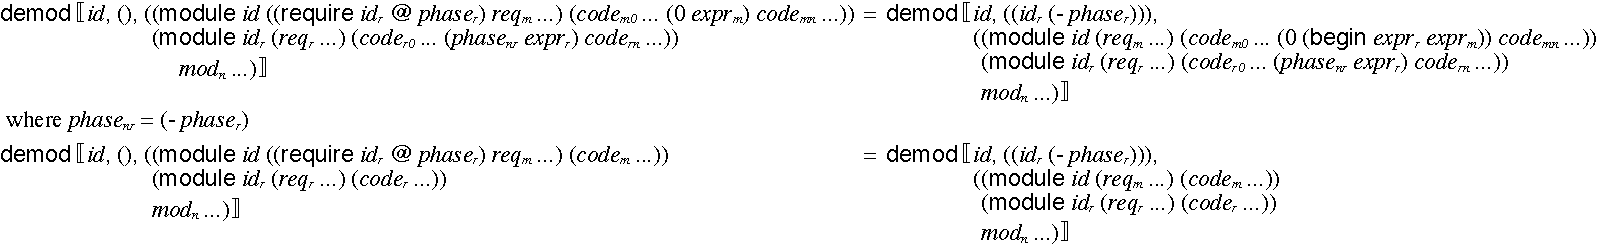
\includegraphics[width=\textwidth]{figures/demod-redex1}
\caption{Demodularization algorithm}
\label{fig:demod-redex1}
\end{figure}
The rules in Figure~\ref{fig:demod-redex1} apply when the main module requires the next module in the module list.
Both rules add the required module's \emph{id} to the working list of required modules so that the algorithm will follow the complete require graph.
% TODO: check to see if there is a diamond pattern, will the algorithm handle it correctly (I don't think it will right now)
The first rule handles the case where the required module has code that will be at phase 0 for the main module and puts that code before the existing phase 0 code of the main module.
\begin{figure}[!h]
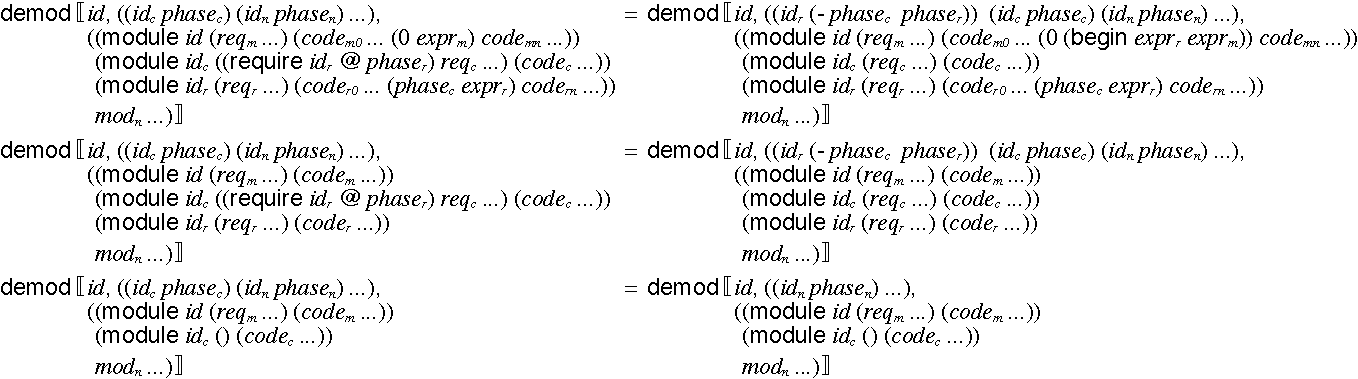
\includegraphics[width=\textwidth]{figures/demod-redex2}
\caption{Demodularization algorithm}
\label{fig:demod-redex2}
\end{figure}
The rules in Figure~\ref{fig:demod-redex2} apply when handling the working list of required modules. 
The first rule is similar to the first rule of Figure~\ref{fig:demod-redex1} because it extracts code that will be in phase 0 of the main module and inserts it into the main module.
The second rule handles the case where there is no matching code for phase 0.
The third rule removes an entry from the working list when the module has no more requires.

\begin{figure}[!h]
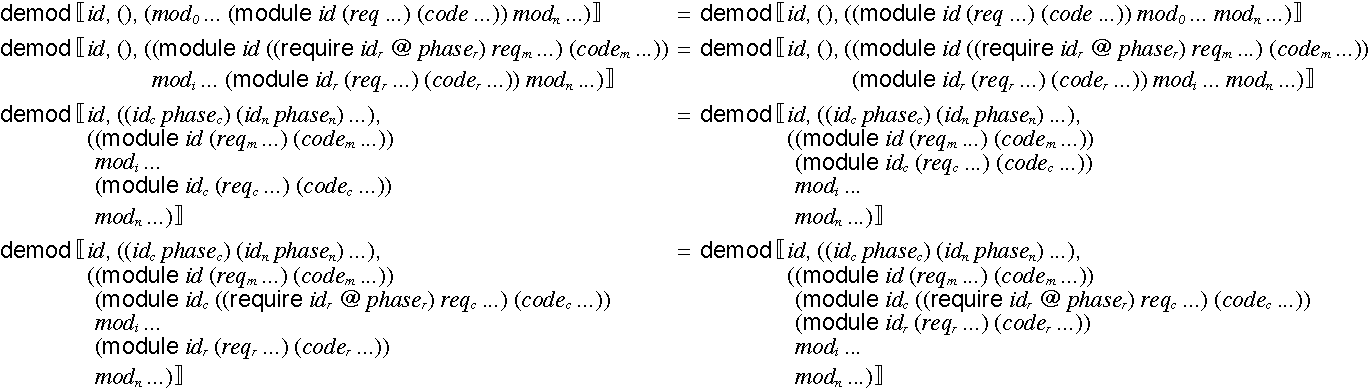
\includegraphics[width=\textwidth]{figures/demod-redex3}
\caption{Demodularization algorithm}
\label{fig:demod-redex3}
\end{figure}

The final four rules in Figure~\ref{fig:demod-redex3} rearrange the program's module list so that modules that require each other are adjacent in the list and the other rules can apply.

\section{Equivalence}
We claim that the programs will evaluate to the same answers before and after demodularization. 

\newtheorem*{theorem}{Theorem}
\begin{theorem}
Evaluating a program P a number of steps n and the demodularized program $P'$ a number of steps m will be bisimilar with respect to the stores of the programs as shown in Figure~\ref{fig:bisim.tex}.
\end{theorem}

\begin{figure}[h]
  \centering
  \begin{tikzpicture}
\node (P) at (0,0) {$P$};
\node [right=of P] (P') {$P'$};
\node [below=of P] (Phat) {$\hat{P}$};
\node [below=of P'] (P'hat) {$\hat{P'}$};
\draw[<->] (P)--(P');
\draw[<->] (Phat)--(P'hat);
\draw[->]  (P)--(Phat) node [midway,left] {$n$};
\draw[->]  (P')--(P'hat) node [midway,right] {$m$};
\end{tikzpicture}

  \caption{Bisimulation of a program before and after demodularization}
  \label{fig:bisim.tex}
\end{figure}

% Properties: grab all code should grab, never grab extra code, renaming doesn't clash

\begin{proof}[Proof Sketch]
The proof is by induction on the DAG of required modules in a program.
For each shape of possible requires in a program, we would show the evaluation before and after demodularization run the same module code in the same order and result in the same stores.
\end{proof}

The full proof of the theorem would not be instructive because of the complexities of the implementation of the model and the demodularization algorithm.

